\documentclass[t,12pt]{beamer}

\usepackage{pgfpages}
%\setbeameroption{show notes on second screen=left}

\usepackage{graphicx}

\hypersetup{colorlinks=true,linkcolor=blue,urlcolor=blue}

\usetheme{metropolis}
\title{R and its History}
\date{\today}
\author{Wolfgang Viechtbauer}
\institute{Maastricht University}

\graphicspath{{images/}}

\begin{document}

\maketitle

%%%%%%%%%%%%%%%%%%%%%%%%%%%%%%%%%%%%%%%%%%%%%%%%%%%%%%%%%%%%%%%%%%%%%%%%%%%%%%%

\begin{frame}{What is R?}

\begin{itemize}
   \item R is a system for data manipulation, statistical and numerical analysis, and graphical display
   \item freely available under the GNU General Public License (GPL) → open-source
   \item runs under Windows, MacOS, Unix/Linux, and even on Android! (and with some tricks also on iOS) -- \\ but why would you???
   \item now a bit of history ...
\end{itemize}

\end{frame}

%%%%%%%%%%%%%%%%%%%%%%%%%%%%%%%%%%%%%%%%%%%%%%%%%%%%%%%%%%%%%%%%%%%%%%%%%%%%%%%

{
\usebackgroundtemplate{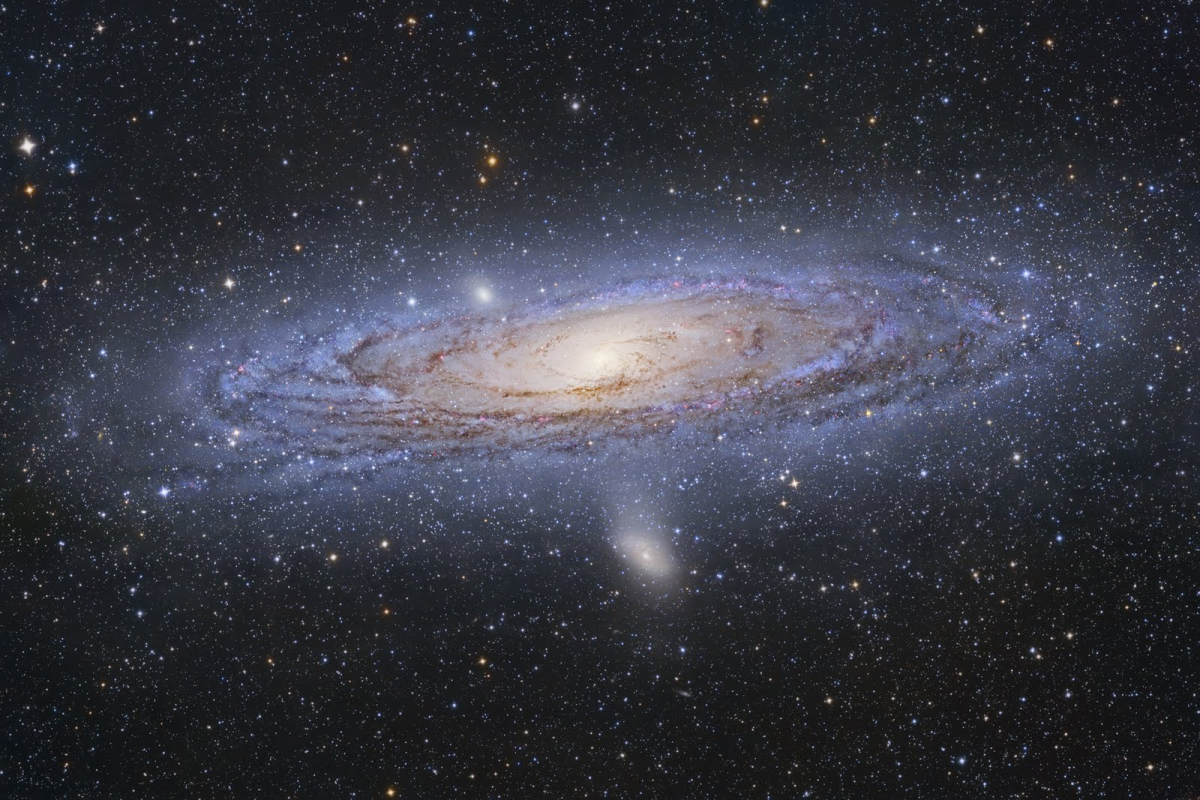
\includegraphics[width=\paperwidth,height=\paperheight]{milkyway.png}}
\begin{frame}

\note[item]{13.82 billion years ago, the universe was formed}

\end{frame}
}

%%%%%%%%%%%%%%%%%%%%%%%%%%%%%%%%%%%%%%%%%%%%%%%%%%%%%%%%%%%%%%%%%%%%%%%%%%%%%%%

\begin{frame}{History of S and R}

\begin{center}
... it began May 5, 1976 at:

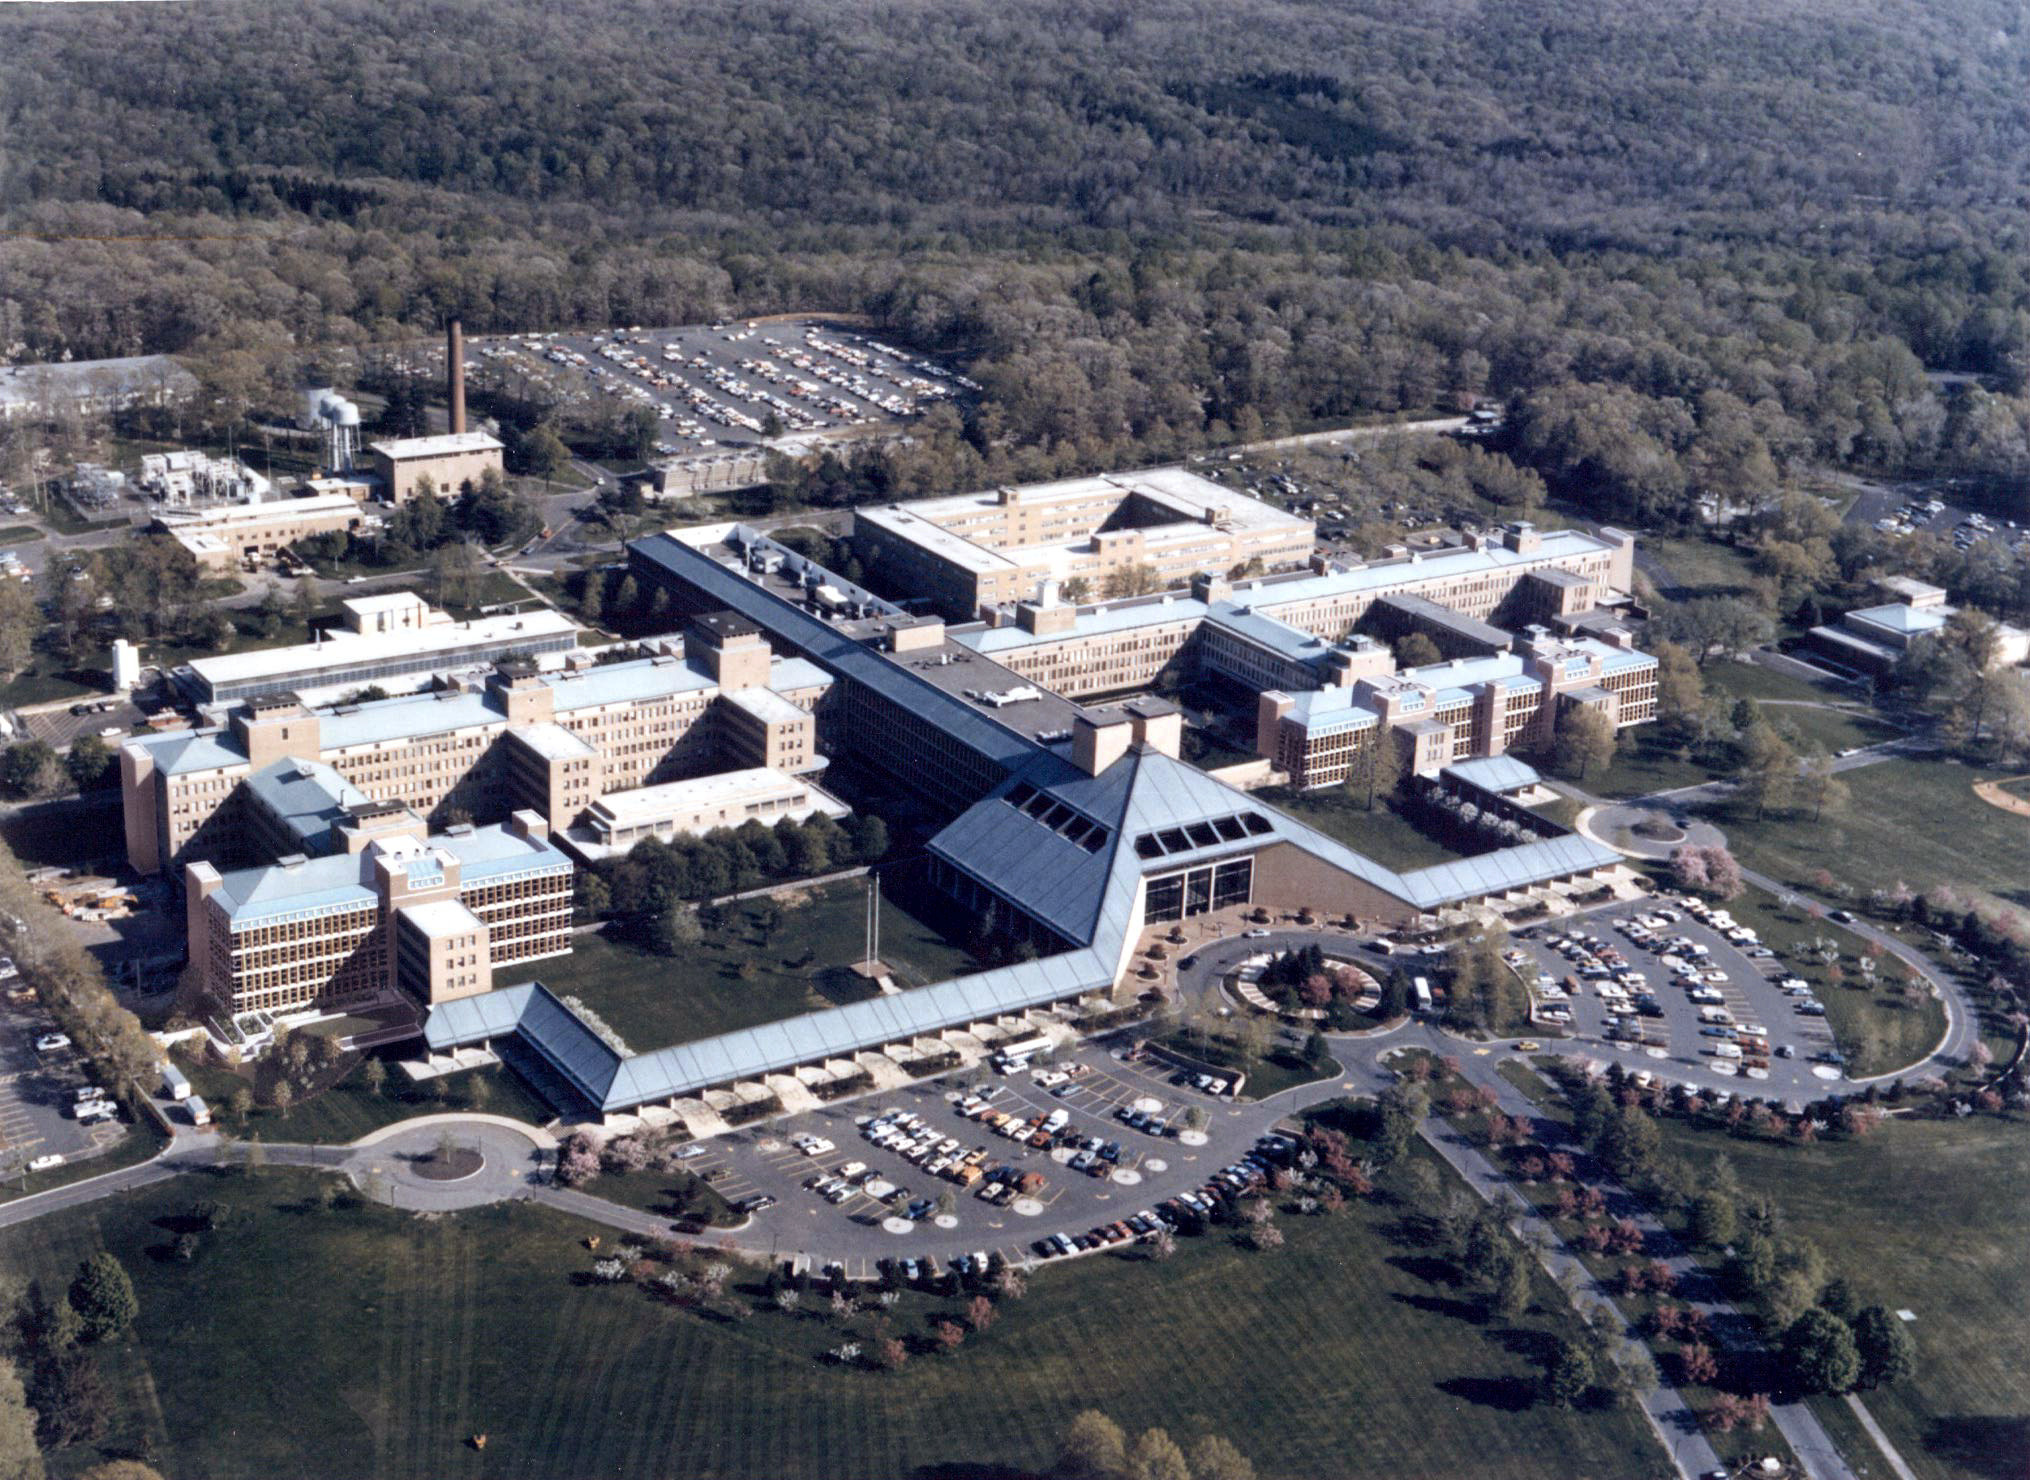
\includegraphics[width=0.75\textwidth]{belllabs.jpg} \\
\href{http://en.wikipedia.org/wiki/Bell_Labs}{Bell Laboratories}, Murray Hill, New Jersey
\end{center}

\note[item]{bell labs is a research subsidiary of Alcatel-Lucent and formerly of AT\&T}
\note[item]{lots of novel things were generated at bell labs (e.g., radio astronomy, the transistor, the laser, the operating system UNIX, the programming languages C and C++)}

\end{frame}

%%%%%%%%%%%%%%%%%%%%%%%%%%%%%%%%%%%%%%%%%%%%%%%%%%%%%%%%%%%%%%%%%%%%%%%%%%%%%%%

\begin{frame}{History of S and R}

\begin{columns}

\column{0.60\textwidth}

\begin{itemize}
   \item informal meeting to discuss development of a new system for statistical computing
   \item first implementation made by Rick Becker \& \href{http://en.wikipedia.org/wiki/John_Chambers_(programmer)}{John Chambers} (and a few others)
   \item called "the system"
\end{itemize}

\column{0.30\textwidth}

\begin{center}
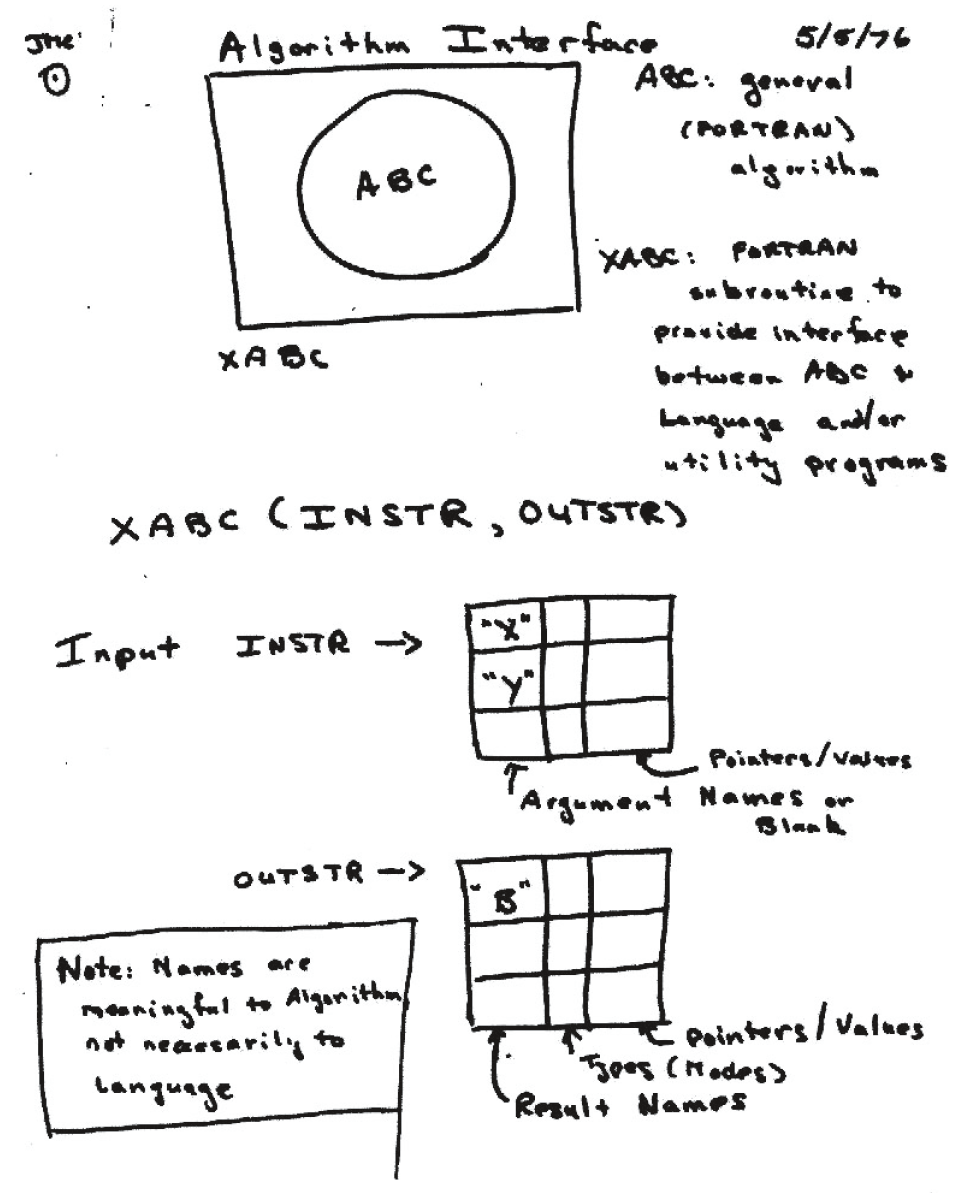
\includegraphics[width=\textwidth]{sketch.png} \\
\tiny
\textit{sketch of the system design \\ made on the first meeting}
\end{center}

\end{columns}

\end{frame}

%%%%%%%%%%%%%%%%%%%%%%%%%%%%%%%%%%%%%%%%%%%%%%%%%%%%%%%%%%%%%%%%%%%%%%%%%%%%%%%

\begin{frame}{History of S and R}

\begin{itemize}
   \item ``the system'' → ``\href{http://en.wikipedia.org/wiki/S_(programming_language)}{S}'' (the S language) (also play on name of programming languages, such as C)
   \item first UNIX version of S in 1979 (version 2)
   \item distributed outside Bell Labs in 1980
   \item source code released in 1981, but licensed in 1984 for educational and commercial purposes
\end{itemize}

\end{frame}

%%%%%%%%%%%%%%%%%%%%%%%%%%%%%%%%%%%%%%%%%%%%%%%%%%%%%%%%%%%%%%%%%%%%%%%%%%%%%%%

\begin{frame}{History of S and R}

\begin{itemize}
   \item Becker \& Chambers (1984). \textit{S: An Interactive Environment for Data Analysis and Graphics}.
   \item Becker \& Chambers (1985). \textit{Extending the S System}.
   \item Becker, Chambers, \& Wilks (1988): \textit{The New S Language: A Programming Environment for Data Analysis and Graphics}.
   \item Chambers \& Hastie (1991). \textit{Statistical Models in S}.
   \item Chambers (1998). \textit{Programming with Data: A Guide to the S Language}.
\end{itemize}

\end{frame}

%%%%%%%%%%%%%%%%%%%%%%%%%%%%%%%%%%%%%%%%%%%%%%%%%%%%%%%%%%%%%%%%%%%%%%%%%%%%%%%

\begin{frame}{History of S and R}

\begin{itemize}
   \item \href{http://en.wikipedia.org/wiki/S-plus}{S-PLUS}, a commercial implementation of S, released in 1988 by Statistical Sciences, Inc. (now TIBCO)
   \item \href{http://en.wikipedia.org/wiki/Ross_Ihaka}{Ross Ihaka} and \href{http://en.wikipedia.org/wiki/Robert_Gentleman_(statistician)}{Robert Gentleman} start developing a statistical programming language "not unlike S" at the University of Auckland in the 1990s
\end{itemize}

\begin{center}
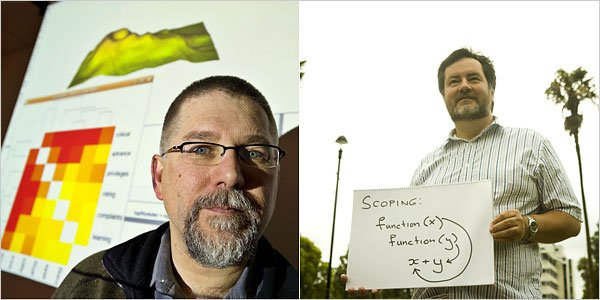
\includegraphics[width=0.75\textwidth]{ihaka_gentleman.jpg}
\end{center}

\end{frame}

%%%%%%%%%%%%%%%%%%%%%%%%%%%%%%%%%%%%%%%%%%%%%%%%%%%%%%%%%%%%%%%%%%%%%%%%%%%%%%%

\begin{frame}{Some R Milestones}

\begin{itemize}
   \item first binary of R released in 1993
   \item Ihaka, R., \& Gentleman, R. (1996). R: A language for data analysis and graphics. \textit{Journal of Computational and Graphical Statistics, 5}(3), 299--314.
   \item source code released in 1997 (\href{https://cran.r-project.org/}{CRAN} is started)
   \item \href{http://www.r-project.org/contributors.html}{R Core group} formed in 1997 with 9 members, now 20
   \item version 1.0.0 (2000), version 2.0.0 (2004)
   \item first \href{http://www.r-project.org/conferences.html}{useR! conference} in May 2004 in Vienna, Austria
   \item version 3.0.0 released April 2013
\end{itemize}

\end{frame}

%%%%%%%%%%%%%%%%%%%%%%%%%%%%%%%%%%%%%%%%%%%%%%%%%%%%%%%%%%%%%%%%%%%%%%%%%%%%%%%

\begin{frame}{MoRe Milestones}

\begin{itemize}
   \item new \href{https://www.r-project.org/}{website} and logo in 2015:
\end{itemize}

\begin{columns}

\column{0.45\textwidth}

\begin{center}

\includegraphics[scale=0.43]{rlogo_old.png}
\end{center}

\column{0.45\textwidth}

\begin{center}

\includegraphics[scale=0.10]{rlogo_new.png}
\end{center}

\end{columns}

\begin{columns}

\column{0.45\textwidth}

\begin{center}
\textit{the old one}
\end{center}

\column{0.45\textwidth}

\begin{center}
\textit{the new one}
\end{center}

\end{columns}

\vspace{0.5cm}

\begin{itemize}
   \item current version: R 3.4.2 released September 2017
\end{itemize}

\end{frame}

%%%%%%%%%%%%%%%%%%%%%%%%%%%%%%%%%%%%%%%%%%%%%%%%%%%%%%%%%%%%%%%%%%%%%%%%%%%%%%%

\begin{frame}{Other Related Developments}

\begin{itemize}
   \item \href{https://en.wikipedia.org/wiki/Revolution_Analytics}{Revolution Analytics} founded in 2007 (now Microsoft)
   \item \href{http://www.rstudio.com/}{RStudio} founded in 2008
   \item \href{http://www.nytimes.com/2009/01/07/technology/business-computing/07program.html}{New York Times article} about R in January 2009
   \item \href{https://www.r-consortium.org/}{R Consortium} founded in 2015
   \item \href{http://en.wikipedia.org/wiki/Big_data}{big data} (Oracle, IBM, Intel, Microsoft, ...)
   \item \href{http://en.wikipedia.org/wiki/Data_science}{data science} (`hacking' skills core component)
   \item web-based interactive graphics/dashboards (\href{http://shiny.rstudio.com/}{shiny}, \href{http://cran.r-project.org/web/packages/googleVis/index.html}{googleVis}, \href{http://rmarkdown.rstudio.com/flexdashboard/}{flexdashboard}, \href{http://www.htmlwidgets.org/}{htmlwidgets}, \href{https://plot.ly/r/}{plotly + R}, ...)
   \item \href{http://en.wikipedia.org/wiki/Open_science}{open science}, \href{http://en.wikipedia.org/wiki/Reproducibility}{reproducible research}
   \item \href{http://rmarkdown.rstudio.com/}{rmarkdown} (easy creation of dynamic documents, presentations, and reports from R)
\end{itemize}

\note[item]{Revolution Analytics was acquired by Microsoft in April 2015}

\end{frame}

%%%%%%%%%%%%%%%%%%%%%%%%%%%%%%%%%%%%%%%%%%%%%%%%%%%%%%%%%%%%%%%%%%%%%%%%%%%%%%%

\begin{frame}{Why is it called R?}

\begin{itemize}
   \item \textbf{R}oss Ihaka and \textbf{R}obert Gentleman
   \item pun/play on the name of the S language
   \item like computer scientists, statisticians are geeks
   \item<2-> \href{https://hbr.org/2012/10/data-scientist-the-sexiest-job-of-the-21st-century/}{Data Scientist: The Sexiest Job of the 21st Century}
\end{itemize}

\end{frame}

%%%%%%%%%%%%%%%%%%%%%%%%%%%%%%%%%%%%%%%%%%%%%%%%%%%%%%%%%%%%%%%%%%%%%%%%%%%%%%%

\begin{frame}{Modes of Interacting with R}

\begin{itemize}
   \item \textit{\textbf{interactively}}: type commands into the R console and get immediate feedback
   \begin{itemize}
      \item to use R as a ``calculator on speed''
      \item useful for spontaneous exploration of data
      \item to test parts of a script file
   \end{itemize}
   \item \textit{\textbf{via script files}}: type commands into a script file and then do one of the following:
   \begin{itemize}
      \item copy-paste commands to execute into the R console
      \item read in and execute commands with \texttt{source()}
      \item batch processing (source file from command line)
   \end{itemize}
\end{itemize}

\end{frame}

%%%%%%%%%%%%%%%%%%%%%%%%%%%%%%%%%%%%%%%%%%%%%%%%%%%%%%%%%%%%%%%%%%%%%%%%%%%%%%%

\begin{frame}{Script Files}

\begin{itemize}
   \item promotes:
   \begin{itemize}
      \item organized programming/analyses
      \item code sharing and reuse
   \end{itemize}
   \item increases replicability
   \item can write/edit script files with:
   \begin{itemize}
      \item built-in editor
      \item external editor
      \item \href{https://en.wikipedia.org/wiki/Integrated_development_environment}{integrated development environment} (IDE)
   \end{itemize}
\end{itemize}

\end{frame}

%%%%%%%%%%%%%%%%%%%%%%%%%%%%%%%%%%%%%%%%%%%%%%%%%%%%%%%%%%%%%%%%%%%%%%%%%%%%%%%

\begin{frame}{RStudio}

\begin{itemize}
   \item \href{https://www.rstudio.com/}{RStudio}: an IDE for R
   \item open source (commercial version also available)
   \item runs on Windows, MacOS, and Linux (also via web)
   \item some of the useful features:
   \begin{itemize}
      \item syntax highlighting
      \item code completion
      \item bracket matching
      \item object list and command history
      \item organized workspace (editor, console, plots, …)
   \end{itemize}
\end{itemize}

\end{frame}

%%%%%%%%%%%%%%%%%%%%%%%%%%%%%%%%%%%%%%%%%%%%%%%%%%%%%%%%%%%%%%%%%%%%%%%%%%%%%%%

\begin{frame}{How We Will Proceed ...}

\begin{itemize}
   \item \href{https://cran.r-project.org/}{install R} (if you have not done this yet)
   \item for those new to R, use \href{https://www.rstudio.com/}{RStudio} (install this as well)
   \item hands-on tutorial based on script file on \href{https://wviechtb.github.io/scrum-club/materials/materials.html}{website}
   \item if you have questions, please ask!
\end{itemize}

\end{frame}

%%%%%%%%%%%%%%%%%%%%%%%%%%%%%%%%%%%%%%%%%%%%%%%%%%%%%%%%%%%%%%%%%%%%%%%%%%%%%%%

\end{document}
